%%%%%%%%%%%%%%%%%%%%%%%%%%%%%%%%%%%%%%%%%%%%%%%%%%%%%%%%%%%%%%%%%%%%%%%%%%%%%%%%
%Tutorial slides on Python.
%
% Author: FOSSEE
% Copyright (c) 2009, FOSSEE, IIT Bombay
%%%%%%%%%%%%%%%%%%%%%%%%%%%%%%%%%%%%%%%%%%%%%%%%%%%%%%%%%%%%%%%%%%%%%%%%%%%%%%%%

\documentclass[14pt,compress]{beamer}
%\documentclass[draft]{beamer}
%\documentclass[compress,handout]{beamer}
%\usepackage{pgfpages} 
%\pgfpagesuselayout{2 on 1}[a4paper,border shrink=5mm]

% Modified from: generic-ornate-15min-45min.de.tex
\mode<presentation>
{
  \usetheme{Warsaw}
  \useoutertheme{infolines}
  \setbeamercovered{transparent}
}

\usepackage[english]{babel}
\usepackage[latin1]{inputenc}
%\usepackage{times}
\usepackage[T1]{fontenc}

% Taken from Fernando's slides.
\usepackage{ae,aecompl}
\usepackage{mathpazo,courier,euler}
\usepackage[scaled=.95]{helvet}
\usepackage{amsmath}

\definecolor{darkgreen}{rgb}{0,0.5,0}

\usepackage{listings}
\lstset{language=Python,
    basicstyle=\ttfamily\bfseries,
    commentstyle=\color{red}\itshape,
  stringstyle=\color{darkgreen},
  showstringspaces=false,
  keywordstyle=\color{blue}\bfseries}

%%%%%%%%%%%%%%%%%%%%%%%%%%%%%%%%%%%%%%%%%%%%%%%%%%%%%%%%%%%%%%%%%%%%%%
% Macros
\setbeamercolor{emphbar}{bg=blue!20, fg=black}
\newcommand{\emphbar}[1]
{\begin{beamercolorbox}[rounded=true]{emphbar} 
      {#1}
 \end{beamercolorbox}
}
\newcounter{time}
\setcounter{time}{0}
\newcommand{\inctime}[1]{\addtocounter{time}{#1}{\tiny \thetime\ m}}

\newcommand{\typ}[1]{\lstinline{#1}}

\newcommand{\kwrd}[1]{ \texttt{\textbf{\color{blue}{#1}}}  }

%%% This is from Fernando's setup.
% \usepackage{color}
% \definecolor{orange}{cmyk}{0,0.4,0.8,0.2}
% % Use and configure listings package for nicely formatted code
% \usepackage{listings}
% \lstset{
%    language=Python,
%    basicstyle=\small\ttfamily,
%    commentstyle=\ttfamily\color{blue},
%    stringstyle=\ttfamily\color{orange},
%    showstringspaces=false,
%    breaklines=true,
%    postbreak = \space\dots
% }

%%%%%%%%%%%%%%%%%%%%%%%%%%%%%%%%%%%%%%%%%%%%%%%%%%%%%%%%%%%%%%%%%%%%%%
% Title page
\title[Solving Equations \& ODEs]{Python for Science and Engg:\\Solving Equations \& ODEs}

\author[FOSSEE] {FOSSEE}

\institute[IIT Bombay] {Department of Aerospace Engineering\\IIT Bombay}
\date[] {02 April, 2010\\Day 1, Session 6}
%%%%%%%%%%%%%%%%%%%%%%%%%%%%%%%%%%%%%%%%%%%%%%%%%%%%%%%%%%%%%%%%%%%%%%

%\pgfdeclareimage[height=0.75cm]{iitmlogo}{iitmlogo}
%\logo{\pgfuseimage{iitmlogo}}


%% Delete this, if you do not want the table of contents to pop up at
%% the beginning of each subsection:
\AtBeginSubsection[]
{
  \begin{frame}<beamer>
    \frametitle{Outline}
    \tableofcontents[currentsection,currentsubsection]
  \end{frame}
}

\AtBeginSection[]
{
  \begin{frame}<beamer>
    \frametitle{Outline}
    \tableofcontents[currentsection,currentsubsection]
  \end{frame}
}

% If you wish to uncover everything in a step-wise fashion, uncomment
% the following command: 
%\beamerdefaultoverlayspecification{<+->}

%\includeonlyframes{current,current1,current2,current3,current4,current5,current6}

%%%%%%%%%%%%%%%%%%%%%%%%%%%%%%%%%%%%%%%%%%%%%%%%%%%%%%%%%%%%%%%%%%%%%%
% DOCUMENT STARTS
\begin{document}

\begin{frame}
  \maketitle
\end{frame}

%% \begin{frame}
%%   \frametitle{Outline}
%%   \tableofcontents
%%   % You might wish to add the option [pausesections]
%% \end{frame}

\section{Solving linear equations}

\begin{frame}[fragile]
\frametitle{Solution of equations}
Consider,
  \begin{align*}
    3x + 2y - z  & = 1 \\
    2x - 2y + 4z  & = -2 \\
    -x + \frac{1}{2}y -z & = 0
  \end{align*}
Solution:
  \begin{align*}
    x & = 1 \\
    y & = -2 \\
    z & = -2
  \end{align*}
\end{frame}

\begin{frame}[fragile]
\frametitle{Solving using Matrices}
Let us now look at how to solve this using \kwrd{matrices}
  \begin{lstlisting}
    In []: A = array([[3,2,-1],
                      [2,-2,4],                   
                      [-1, 0.5, -1]])
    In []: b = array([1, -2, 0])
    In []: x = solve(A, b)
  \end{lstlisting}
\end{frame}

\begin{frame}[fragile]
\frametitle{Solution:}
\begin{lstlisting}
In []: x
Out[]: array([ 1., -2., -2.])
\end{lstlisting}
\end{frame}

\begin{frame}[fragile]
\frametitle{Let's check!}
\begin{lstlisting}
In []: Ax = dot(A, x)
In []: Ax
Out[]: array([  1.00000000e+00,  -2.00000000e+00,  -1.11022302e-16])
\end{lstlisting}
\begin{block}{}
The last term in the matrix is actually \alert{0}!\\
We can use \kwrd{allclose()} to check.
\end{block}
\begin{lstlisting}
In []: allclose(Ax, b)
Out[]: True
\end{lstlisting}
\inctime{15}
\end{frame}

\subsection{Exercises}

\begin{frame}[fragile]
\frametitle{Problem}
Solve the set of equations:
\begin{align*}
  x + y + 2z -w & = 3\\
  2x + 5y - z - 9w & = -3\\
  2x + y -z + 3w & = -11 \\
  x - 3y + 2z + 7w & = -5\\
\end{align*}
\inctime{10}
\end{frame}

\begin{frame}[fragile]
\frametitle{Solution}
Use \kwrd{solve()}
\begin{align*}
  x & = -5\\
  y & = 2\\
  z & = 3\\
  w & = 0\\
\end{align*}
\end{frame}

\section{Finding Roots}

\begin{frame}[fragile]
\frametitle{Scipy Methods - \typ{roots}}
\begin{itemize}
\item Calculates the roots of polynomials
\item To calculate the roots of $x^2-5x+6$ 
\end{itemize}
\begin{lstlisting}
  In []: coeffs = [1, -5, 6]
  In []: roots(coeffs)
  Out[]: array([3., 2.])
\end{lstlisting}
\vspace*{-.2in}
\begin{center}
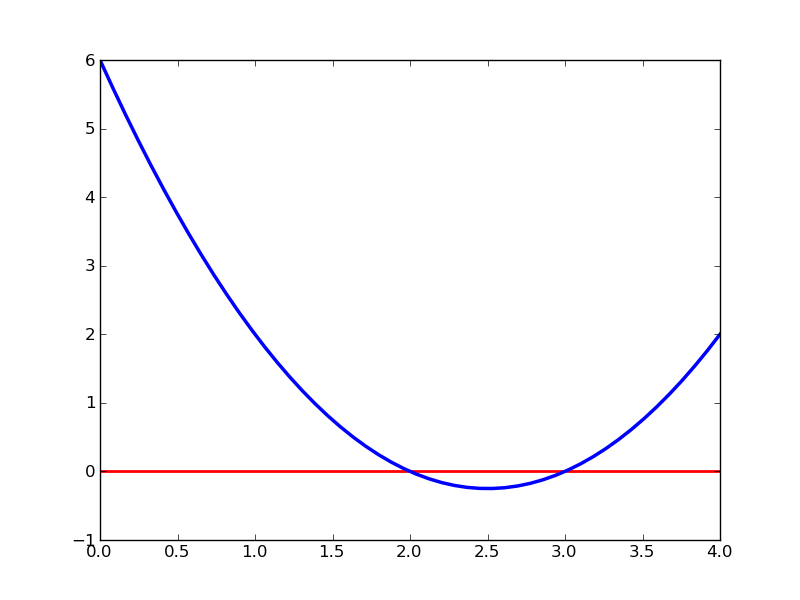
\includegraphics[height=1.6in, interpolate=true]{data/roots}    
\end{center}
\end{frame}

\begin{frame}[fragile]
\frametitle{Scipy Methods - \typ{fsolve}}
\begin{small}
\begin{lstlisting}
  In []: from scipy.optimize import fsolve
\end{lstlisting}
\end{small}
\begin{itemize}
\item Finds the roots of a system of non-linear equations
\item Input arguments - Function and initial estimate
\item Returns the solution
\end{itemize}
\end{frame}

\begin{frame}[fragile]
\frametitle{\typ{fsolve}}
Find the root of $sin(z)+cos^2(z)$ nearest to $0$
\vspace{-0.1in}
\begin{center}
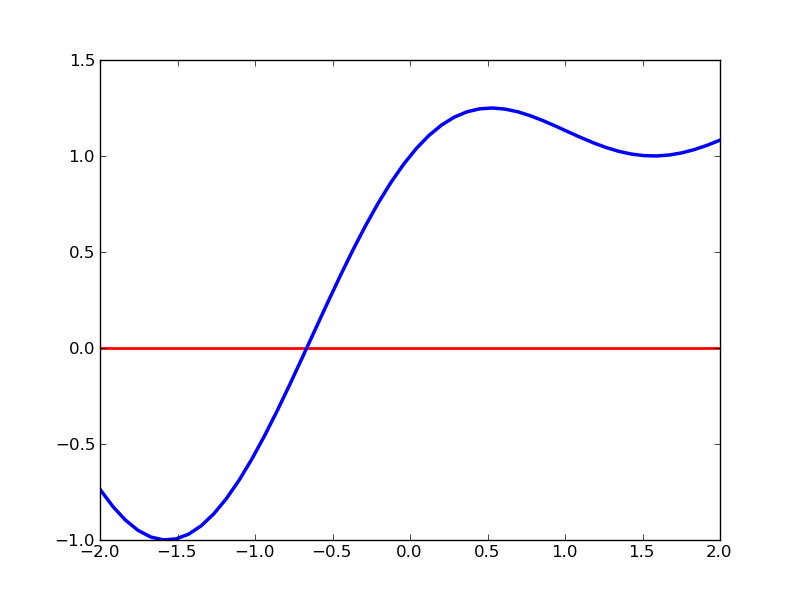
\includegraphics[height=2.8in, interpolate=true]{data/fsolve}    
\end{center}
\end{frame}

\begin{frame}[fragile]
\frametitle{\typ{fsolve}}
Root of $sin(z)+cos^2(z)$ nearest to $0$
\begin{lstlisting}
In []: fsolve(sin(z)+cos(z)*cos(z), 0)
NameError: name 'z' is not defined
\end{lstlisting}
\end{frame}

\begin{frame}[fragile]
\frametitle{\typ{fsolve}}
\begin{lstlisting}
In []: z = linspace(-pi, pi)
In []: fsolve(sin(z)+cos(z)*cos(z), 0)
\end{lstlisting}
\begin{small}
\alert{\typ{TypeError:}}
\typ{'numpy.ndarray' object is not callable}
\end{small}
\end{frame}

\begin{frame}[fragile]
\frametitle{Functions - Definition}
We have been using them all along. Now let's see how to define them.
\begin{lstlisting}
In []: def f(z):
           return sin(z)+cos(z)*cos(z)
\end{lstlisting}
\begin{itemize}
\item \typ{def}
\item name
\item arguments
\item \typ{return}
\end{itemize}
\end{frame}

\begin{frame}[fragile]
\frametitle{Functions - Calling them}
\begin{lstlisting}
In []: f()
---------------------------------------
\end{lstlisting}
\alert{\typ{TypeError:}}\typ{f() takes exactly 1 argument}
\typ{(0 given)}
\begin{lstlisting}
In []: f(0)
Out[]: 1.0
In []: f(1)
Out[]: 1.1333975665343254
\end{lstlisting}
More on Functions later \ldots
\end{frame}

\begin{frame}[fragile]
\frametitle{\typ{fsolve} \ldots}
Find the root of $sin(z)+cos^2(z)$ nearest to $0$
\begin{lstlisting}
In []: fsolve(f, 0)
Out[]: -0.66623943249251527
\end{lstlisting}
\begin{center}
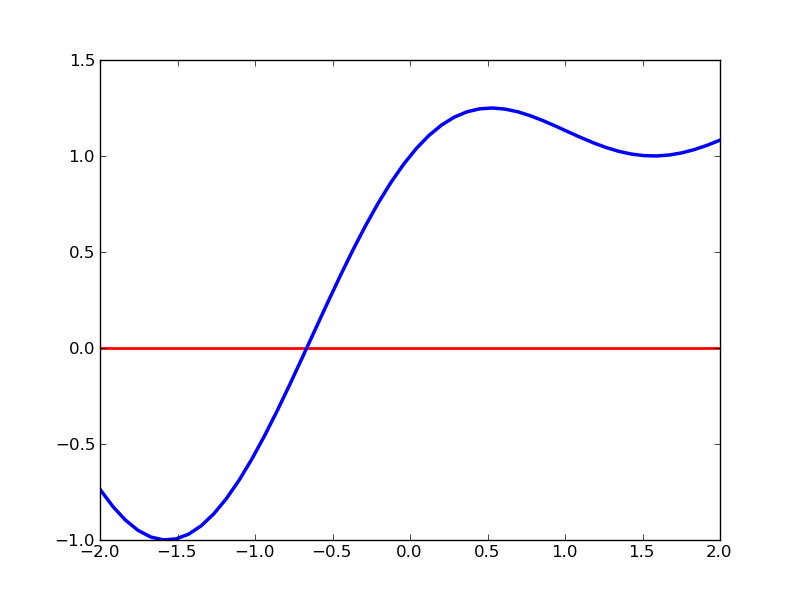
\includegraphics[height=2in, interpolate=true]{data/fsolve}    
\end{center}
\end{frame}

\begin{frame}[fragile]
  \frametitle{Exercise Problem}
  Find the root of the equation $x^2 - sin(x) + cos^2(x) == tan(x)$ nearest to $0$
\end{frame}

\begin{frame}[fragile]
  \frametitle{Solution}
  \begin{small}
  \begin{lstlisting}
def f(x):
    return x**2 - sin(x) + cos(x)*cos(x) - tan(x)
fsolve(f, 0)
  \end{lstlisting}
  \end{small}
  \begin{center}
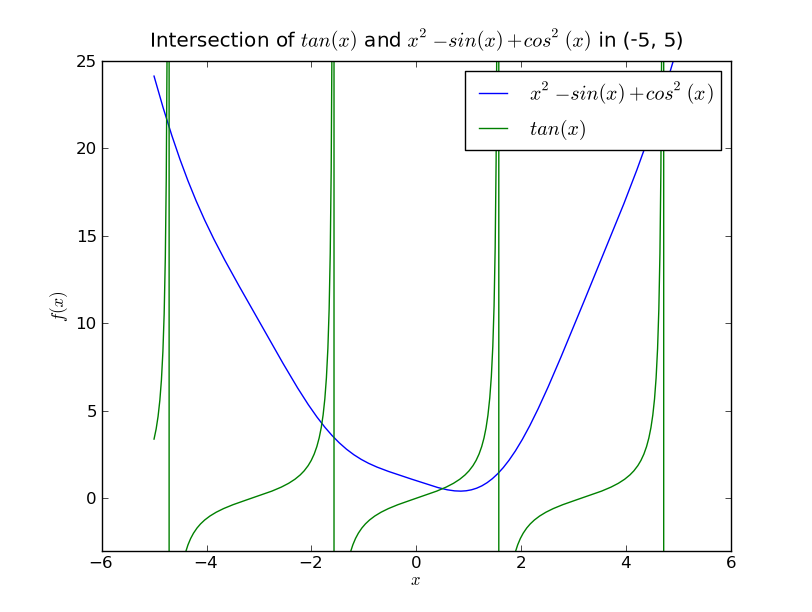
\includegraphics[height=2in, interpolate=true]{data/fsolve_tanx}
  \end{center}
\end{frame}

%% \begin{frame}[fragile]
%% \frametitle{Scipy Methods \dots}
%% \begin{small}
%% \begin{lstlisting}
%% In []: from scipy.optimize import fixed_point

%% In []: from scipy.optimize import bisect

%% In []: from scipy.optimize import newton
%% \end{lstlisting}
%% \end{small}
%% \end{frame}

\section{ODEs}

\begin{frame}[fragile]
\frametitle{Solving ODEs using SciPy}
\begin{itemize}
\item Let's consider the spread of an epidemic in a population
\item $\frac{dy}{dt} = ky(L-y)$ gives the spread of the disease
\item L is the total population.
\item Use L = 25000, k = 0.00003, y(0) = 250
\item Define a function as below
\end{itemize}
\begin{lstlisting}
In []: from scipy.integrate import odeint
In []: def epid(y, t):
  ....     k = 0.00003
  ....     L = 25000
  ....     return k*y*(L-y)
  ....
\end{lstlisting}
\end{frame}

\begin{frame}[fragile]
\frametitle{Solving ODEs using SciPy \ldots}
\begin{lstlisting}
In []: t = linspace(0, 12, 61)

In []: y = odeint(epid, 250, t)

In []: plot(t, y)
\end{lstlisting}
%Insert Plot
\end{frame}

\begin{frame}[fragile]
\frametitle{Result}
\begin{center}
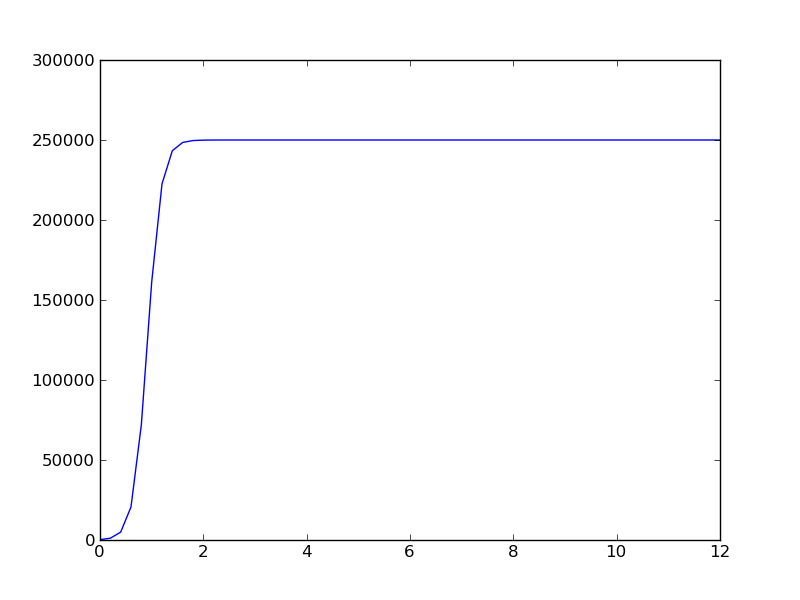
\includegraphics[height=2in, interpolate=true]{data/image}  
\end{center}
\end{frame}


\begin{frame}[fragile]
\frametitle{ODEs - Simple Pendulum}
We shall use the simple ODE of a simple pendulum. 
\begin{equation*}
\ddot{\theta} = -\frac{g}{L}sin(\theta)
\end{equation*}
\begin{itemize}
\item This equation can be written as a system of two first order ODEs
\end{itemize}
\begin{align}
\dot{\theta} &= \omega \\
\dot{\omega} &= -\frac{g}{L}sin(\theta) \\
 \text{At}\ t &= 0 : \nonumber \\
 \theta = \theta_0(10^o)\quad & \&\quad  \omega = 0\ (Initial\ values)\nonumber 
\end{align}
\end{frame}

\begin{frame}[fragile]
\frametitle{ODEs - Simple Pendulum \ldots}
\begin{itemize}
\item Use \typ{odeint} to do the integration
\end{itemize}
\begin{lstlisting}
In []: def pend_int(initial, t):
  ....     theta = initial[0]
  ....     omega = initial[1]
  ....     g = 9.81
  ....     L = 0.2
  ....     f=[omega, -(g/L)*sin(theta)]
  ....     return f
  ....
\end{lstlisting}
\end{frame}

\begin{frame}[fragile]
\frametitle{ODEs - Simple Pendulum \ldots}
\begin{itemize}
\item \typ{t} is the time variable \\ 
\item \typ{initial} has the initial values
\end{itemize}
\begin{lstlisting}
In []: t = linspace(0, 20, 101)
In []: initial = [10*2*pi/360, 0]
\end{lstlisting} 
\end{frame}

\begin{frame}[fragile]
\frametitle{ODEs - Simple Pendulum \ldots}
%%\begin{small}
\typ{In []: from scipy.integrate import odeint}
%%\end{small}
\begin{lstlisting}
In []: pend_sol = odeint(pend_int, 
                         initial,t)
\end{lstlisting}
\end{frame}

\begin{frame}[fragile]
\frametitle{Result}
\begin{center}
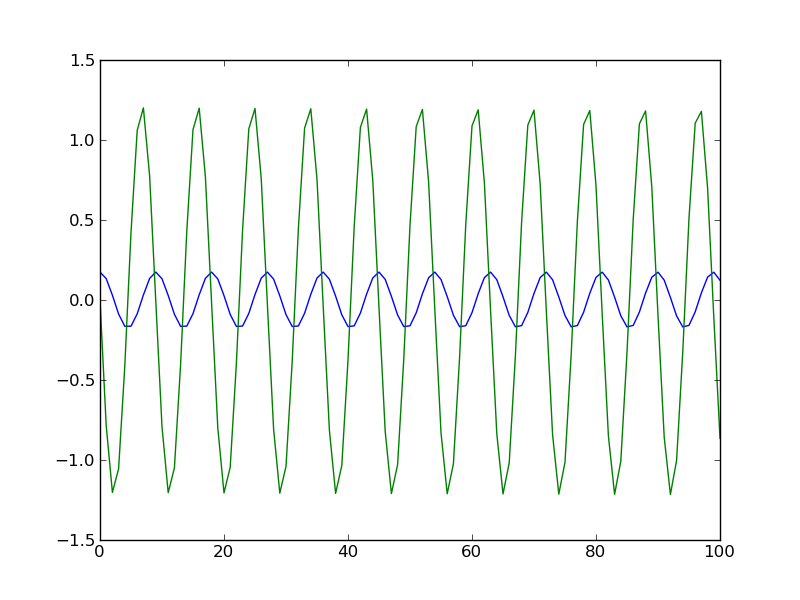
\includegraphics[height=2in, interpolate=true]{data/ode}  
\end{center}
\end{frame}

\begin{frame}
  \frametitle{Things we have learned}
  \begin{itemize}
  \item Solving Linear Equations
  \item Defining Functions
  \item Finding Roots
  \item Solving ODEs
  \end{itemize}
\end{frame}

\end{document}

%% Questions for Quiz %%
%% ------------------ %%

\begin{frame}
\frametitle{\incqno }
Given a 4x4 matrix \texttt{A} and a 4-vector \texttt{b}, what command do
you use to solve for the equation \\
\texttt{Ax = b}?
\end{frame}

\begin{frame}
\frametitle{\incqno }
What command will you use if you wish to integrate a system of ODEs?
\end{frame}

\begin{frame}
\frametitle{\incqno }
How do you calculate the roots of the polynomial, $y = 1 + 6x + 8x^2 +
x^3$?
\end{frame}

\begin{frame}
\frametitle{\incqno }
Two arrays \lstinline+a+ and \lstinline+b+ are numerically almost equal, what command
do you use to check if this is true?
\end{frame}

%% \begin{frame}[fragile]
%% \frametitle{\incqno }
%% \begin{lstlisting}
%%   In []: x = arange(0, 1, 0.25)
%%   In []: print x
%% \end{lstlisting}
%% What will be printed?
%% \end{frame}


%% \begin{frame}[fragile]
%% \frametitle{\incqno }
%% \begin{lstlisting}
%% from scipy.integrate import quad
%% def f(x):
%%     res = x*cos(x)
%% quad(f, 0, 1)
%% \end{lstlisting}
%% What changes will you make to the above code to make it work?
%% \end{frame}

%% \begin{frame}
%% \frametitle{\incqno }
%% What two commands will you use to create and evaluate a spline given
%% some data?
%% \end{frame}

%% \begin{frame}[fragile]
%% \frametitle{\incqno }
%% What would be the result?
%% \begin{lstlisting}
%%   In []: x
%%   array([[0, 1, 2],
%%          [3, 4, 5],
%%          [6, 7, 8]])
%%   In []: x[::-1,:]
%% \end{lstlisting}
%% Hint:
%% \begin{lstlisting}
%%   In []: x = arange(9)
%%   In []: x[::-1]
%%   array([8, 7, 6, 5, 4, 3, 2, 1, 0])
%% \end{lstlisting}
%% \end{frame}

%% \begin{frame}[fragile]
%% \frametitle{\incqno }
%% What would be the result?
%% \begin{lstlisting}
%%   In []: y = arange(3)
%%   In []: x = linspace(0,3,3)
%%   In []: x-y
%% \end{lstlisting}
%% \end{frame}

%% \begin{frame}[fragile]
%% \frametitle{\incqno }
%% \begin{lstlisting}
%%   In []: x
%%   array([[ 0, 1, 2, 3],
%%          [ 4, 5, 6, 7],
%%          [ 8, 9, 10, 11],
%%          [12, 13, 14, 15]])
%% \end{lstlisting}
%% How will you get the following \lstinline+x+?
%% \begin{lstlisting}
%%   array([[ 5, 7],
%%          [ 9, 11]])
%% \end{lstlisting}
%% \end{frame}

%% \begin{frame}[fragile]
%% \frametitle{\incqno }
%% What would be the output?
%% \begin{lstlisting}
%%   In []: y = arange(4)
%%   In []: x = array(([1,2,3,2],[1,3,6,0]))
%%   In []: x + y
%% \end{lstlisting}
%% \end{frame}

%% \begin{frame}[fragile]
%% \frametitle{\incqno }
%% \begin{lstlisting}
%%   In []: line = plot(x, sin(x))
%% \end{lstlisting}
%% Use the \lstinline+set_linewidth+ method to set width of \lstinline+line+ to 2.
%% \end{frame}

%% \begin{frame}[fragile]
%% \frametitle{\incqno }
%% What would be the output?
%% \begin{lstlisting}
%%   In []: x = arange(9)
%%   In []: y = arange(9.)
%%   In []: x == y
%% \end{lstlisting}
%% \end{frame}

